\section{Experiments}
\label{Sec:Exp}
To verify the effectiveness of the proposed network, extensive experiments have been conducted on three datasets. Compared not only with other methods applied in the field of remote sensing image, but also semantic segmentation methods in computer vision field, our network all achieves good performance. The performance of various variants of HF-FCN are also shown below. In this section, the experimental setup is described and the variants of HF-FCN are illustrated.
\subsection{Dataset Description}
a. Massachusetts dataset\par
\setlength{\parindent}{4ex}Massachusetts dataset consists of 151 aerial images of the Boston area which covers roughly 340 square kilometers. The resolution of each image is 1500$\times$ 1500 with the spacial resolution of 1 meter per pixel, composed of red, green and blue channels. This dataset is built by Mnih while ground-truth of the images is produced by Saito et al. This dataset is split into three parts,  a training set of 137 images, a test set of 10 images and validation set of 4 images. To train the network, we create a set of image tiles for training and validation. The detailed description is shown in Table \Rmnum{2}.\par

\setlength{\parindent}{2ex}b. Vaihingen dataset\par
\setlength{\parindent}{4ex}Vaihingen dataset is captured over Vaihingen which is a relatively small village with many detached buildings and small multi story buildings in Germany. This dataset contains 16 labeled images whose spacial resolution is 9cm per pixel. It contains near infra-red, red, green, blue imagery with corresponding normalized digital surface models (nDSMs) and row DSMs. The dataset is divided into training set, validation set and test set which has 11 images, 2 images and 3 images, respectively. The same crop operations are done as the Massachusetts dataset.\par

\setlength{\parindent}{2ex}c. Potsdam dataset\par
\setlength{\parindent}{4ex}In Potsdam dataset, there are 24 labeled images whose ground sampling distance is 5cm. This dataset shows a typical historic city with large building blocks. In order to grasp the global information of the building, we reduced the spacial resolution of the original image from 6000$\times$6000 to 1500$\times$1500. This dataset contains information about 5 channels: red, green, yellow, DSM and nDSM. We split the dataset into training, validation and test sets in proportion to 7${:}$2${:}$1.\par
Data augmentation is made on the dataset b and c. One reason is that methods use the dataset a do not extend the data. To make a fair comparison with other methods, we also do not extend it. Another reason is the data quantity of dataset b and c is not enough. It may lead to inadequate training of our network. Hence, some simple augmentation operations are made in dataset b and c including data rotation and mirror filp. Component of the datasets are shown in Table \Rmnum{2}. Figure 5 shows the sampled patches of dataset a, b, c.\par
\begin{figure}
\centering
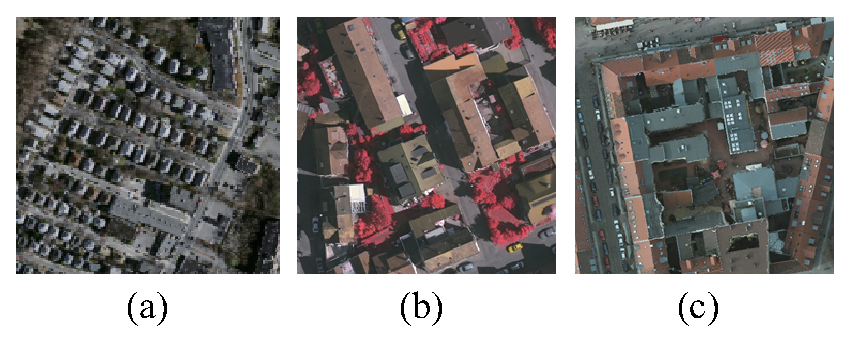
\includegraphics[width=8cm]{Figures/datasets.eps}
\caption{Sample patches on the three datasets  (a) Massachusetts dataset (b) Vaihingen dataset (c) Potsdam dataset}
\label{5}
\end{figure}
\begin{table}
 \centering
 \caption{Composition of dataset}
 \begin{tabular}{c|ccc}
\hline
&Masschusetts&Vaihingen &Potsdam\\  \hline
Labeled images & 151& 16 &24\\ \hline
GSD & 1m & 9cm & 5cm\\ \hline
Bands&R,G,B &IR,R,G,DSM &IR,R,G,B,DSM\\ \hline
%Training set & \tabincell{c}{1,3,5,7,13,\\17,21,23,26,32,37} &\tabincell{c}{2\_10,3\_10,3\_11,3\_12,\\4\_11,4\_12,5\_10,5\_12,\\6\_8,6\_8,6\_10,6\_11,\\6\_12,7\_7,7\_9,7\_11,7\_12}\\ \hline
Training images &137 & 11 & 17\\ \hline
Training patches&75938 &115088 &85000\\ \hline
%validation set & 11,28,34 &2\_11,4\_10,5\_11,7\_10\\ \hline
Validation images & 4 & 3 & 4\\ \hline
validation patches &2500 & 28376 &25000 \\\hline
%Test set & 15,30 &2\_12,6\_7,7\_8 \\ \hline
Test images & 10 & 2 & 3\\ \hline
\end{tabular}
\end {table}
\subsection{Training Settings}
HF-FCN first trained on dataset a because of large amounts of training data. The pre-trained VGG16 Net model is used to finetune our HF-FCN. We Use the stochastic gradient descent algorithm with the learning rate divided by 10 for each 8000 iterations to train our network. The drop-out ratio is set to 0.5 which avoids overfitting. When the HF-FCN converges on the dataset a, we transfer it to the other datasets. All experiments in this paper are performed using the deep learning framework Caffe and train on a single NVIDIA Titan 12GB GPU. The hyper-parameters are listed in Table \Rmnum{3}.
\begin{table}
\centering
\caption {Parameters for Network Training}
\begin{tabular}{c|c|c|c}
\hline
&Massachusetts &Vaihigen &Potsdam\\  \hline
%input size & 256$\times$256 &256$\times$256 \\
mini-bachsize &18& 15 &15 \\
initial learning rate &10$^-5$ & 10$^-6$ &10$^-5$\\
test\_interval&1000 & 1000 &1000\\
%type &SGD &SGD &SGD\\
training iteration &10000 & 10000& 10000\\
momentum&0.9 &0.9 &0.9\\
clip\_gradients &16000& 10000 &10000\\
weight\_decay&0.02& 0.005 &0.005\\ \hline
\end{tabular}
\end{table}

\subsection{Evaluation Metrics}
Some evaluation metrics are adopted in our work. For dataset a, the most common metrics are correctness (precision) and completeness (recall). We use the stantdard precision and recall scores ($\rho$=0) and the relaxed precision and recall scores with $\rho$=3 to evaluate the prediction results. Here the relaxed precision means the predicted pixels are within $\rho$ pixels of a true pixel while the relaxed recall is the true pixels are within $\rho$ pixels of a predicted pixel. The time cost is used to measure the efficiency of our HF-FCN. For dataset b and c, we use correctness, completeness and F1 score as evaluation metrics. \par
\begin{equation}
 {completeness} = \frac{TP}{TP+FN},
\end{equation}
\begin{equation}
{correctness} = \frac{TP}{TP+FP},
\end{equation}
\begin{equation}
{F1\_score}= 2\cdot\frac{completeness\cdot correctness}{completeness+correctness}
\end{equation}

where TP indicates the true positives, FP indicates the false positive, TN indicates the true negatives and FN indicates the false negatives.